\documentclass{article}


% if you need to pass options to natbib, use, e.g.:
% \PassOptionsToPackage{numbers, compress}{natbib}
% before loading nips_2018

% ready for submission
% \usepackage{nips_2018}

% to compile a preprint version, e.g., for submission to arXiv, add
% add the [preprint] option:
\usepackage[final]{nips_2018}
\usepackage{fullpage}

% to compile a camera-ready version, add the [final] option, e.g.:
% \usepackage[final]{nips_2018}

% to avoid loading the natbib package, add option nonatbib:
% \usepackage[nonatbib]{nips_2018}

\usepackage[utf8]{inputenc} % allow utf-8 input
\usepackage[T1]{fontenc}    % use 8-bit T1 fonts
\usepackage{hyperref}       % hyperlinks
\usepackage{url}            % simple URL typesetting
\usepackage{booktabs}       % professional-quality tables
\usepackage{amsfonts}       % blackboard math symbols
\usepackage{amsmath}
\usepackage{nicefrac}       % compact symbols for 1/2, etc.
\usepackage{microtype}      % microtypography
\usepackage[pdftex]{graphicx}
\graphicspath{ {images/} }



\title{Reddit Communities: Exploring Similarities and Conflicts}

% The \author macro works with any number of authors. There are two
% commands used to separate the names and addresses of multiple
% authors: \And and \AND.
%
% Using \And between authors leaves it to LaTeX to determine where to
% break the lines. Using \AND forces a line break at that point. So,
% if LaTeX puts 3 of 4 authors names on the first line, and the last
% on the second line, try using \AND instead of \And before the third
% author name.

\author{
  Davide Spallaccini\thanks{\texttt{spallaccini.1642557@studenti.uniroma1.it}} \\
  Department of Computer, Control \\ and Management Engineering\\
  Sapienza University of Rome\\
  Rome, Italy \\
  \And
  Beatrice Bevilacqua\thanks{\texttt{bevilacqua.1645689@studenti.uniroma1.it}} \\
  Department of Computer, Control \\ and Management Engineering\\
  Sapienza University of Rome\\
  Rome, Italy \\
   \\
  %% examples of more authors
  \And
  Anxhelo Xhebraj\thanks{\texttt{xhebraj.1643777@studenti.uniroma1.it}} \\
  Department of Computer, Control \\ and Management Engineering\\
  Sapienza University of Rome\\
  Rome, Italy
  %% Affiliation \\
  %% Address \\
  %% \texttt{email} \\
  %% \AND
  %% Coauthor \\
  %% Affiliation \\
  %% Address \\
  %% \texttt{email} \\
  %% \And
  %% Coauthor \\
  %% Affiliation \\
  %% Address \\
  %% \texttt{email} \\
  %% \And
  %% Coauthor \\
  %% Affiliation \\
  %% Address \\
  %% \texttt{email} \\
}

\begin{document}
% \nipsfinalcopy is no longer used

\maketitle

\begin{abstract}

  Inspired by the "Community Interaction and Conflict on the Web"
  paper[1] we have analyzed the Reddit social network focusing
  on the content of the comments of its communities to have some insights of
  their interactions and to reproduce some of the results of the authors. We
  have applied novel deep-learning models achieving competitive results,
  reproduced the reply network analysis presented in the paper and confronted
  the difficulties and issues of the design and development of a recommender
  system.

\end{abstract}

\section{Introduction and Related Work}
\label{sec:intro}

Reddit is a growing social network based on communities called
subreddits where users interact by posting articles and links regarding
topics of the community and by commenting them. Interests of communities usually
overlap but the
opinions on the subject matter may diverge. In this context, a user of one
subreddit (source of the link) may post a cross-link (i.e. a link that
points to another subreddit which is the target of the link) and lead to
a mobilization where the users of the source community interact with the users
of the target community in the targeted post. The concept has been explored in
the paper "Community Interaction and Conflict on the Web" in which the authors
have constructed a dataset starting from 40 months of reddit content such as
posts and comments. The resulting dataset is composed of 394,216 instances of
mobilizing cross-links represented as id of source post, id of target post
and a label telling whether the mobilization was neutral/positive ("non-burst")
or negative ("burst").

Starting from the concept of user and community interactions on Reddit we
decided to reproduce some of the results of the paper to have an insight of the
process and understand the difficulties and challenges of the task. Based on the
dataset described above we applied a novel model employing deep learning
concepts,
using a combination of a convolutional neural network followed by an LSTM
recurrent network to predict whether a mobilization is positive or negative,
i.e. whether it will lead to a conflict. Additionally, on the target posts of
the negative mobilizations we analyzed the kinds of user-user interactions
developed by constructing a reply network of the comments for each post and 
applying personalized PageRank. Finally intrigued by the structure of the social
network we decided to find similarities between communities and construct a
recommender system to permit the users to discover new communities based on
their interaction history.

\section{Dataset Retrieval}
\label{sec:retrieval}

The "Community Interaction and Conflict on the Web" dataset is provided in a
preprocessed form where posts are represented by the indices of the word
embeddings of the words forming its title and body and users by a feature vector
that describes the activity levels and lexical features of their previous posts.
In order to have more flexibility over the design choices of our models we
decided to rely on that dataset only as a ground truth and to retrieve the raw
content from the source, i.e. the reddit social network. In particular we used
the Pushshift API in conjunction with the Python Reddit API Wrapper (PRAW). In
this task we encountered our first challenge which was due to the rate limiting
set by both the APIs which allow respectively an average of 120 requests and
60 requests per minute. Moreover to retrieve the necessary data for each
instance of the dataset multiple requests were required. By launching multiple
processes in parallel and using multiple accounts we were able to get the
most of the information needed.

For the LSTM-based classification task, given the post IDs of the sources of
the cross-links provided by the dataset, the Pushshift APIs were used to
retrieve: in a first request the text of the title and of the body of the post,
in a second one the ids of the top 8 comments present in the post and in a third
one the first 512 characters of the body of each comment to avoid giving too
much weight to the comments with respect to post text. The process just
described unfortunately incurred into some exceptions caused by rate limiting
and post deletion but still allowed to collect enough data for the
classification as will be described in Section \ref{sec:davide}.

To reproduce the analysis on the reply network we took only
the instances of the dataset that were labeled as "burst" i.e. the ones that
produced a negative mobilization. For each of the target posts we used the
PRAW library to retrieve its comments and the authors of those comments. Of the
authors, only the subset of users that were attackers or defenders were chosen.
In order to know whether a user is an attacker or defender we used the Pushshift
API to retrieve the comments submitted by the user in the 30 days before the
target post submission. An attacker (resp. defender) is a user who has made at
least one comment in the source (resp. target) subreddit in the 30 days prior to the
cross-link but who did not comment in the target (resp. source) during this time
period.

The gathering of the data for the subreddit similarities and the recommender
system was done by downloading all the comments submitted to reddit in December
2017. The data for each reddit month is available as a lmza compressed file at
\href{files.pushshift.io}{pushshift.io} in JSONLines format which is the
standard for Big Data. In this task we encountered another issue in dataset
retrieval since the size of the uncompressed file reached the size of $\approx
80$GB filling up the available disk space of the machine. We opted for first
performing a counting of comments by subreddit to spot the most active
subreddits represented in Figure \ref{fig:hist} by performing a scan over the
compressed dataset since lzma compression permits streaming decompression.

\begin{figure}[h]
\centering
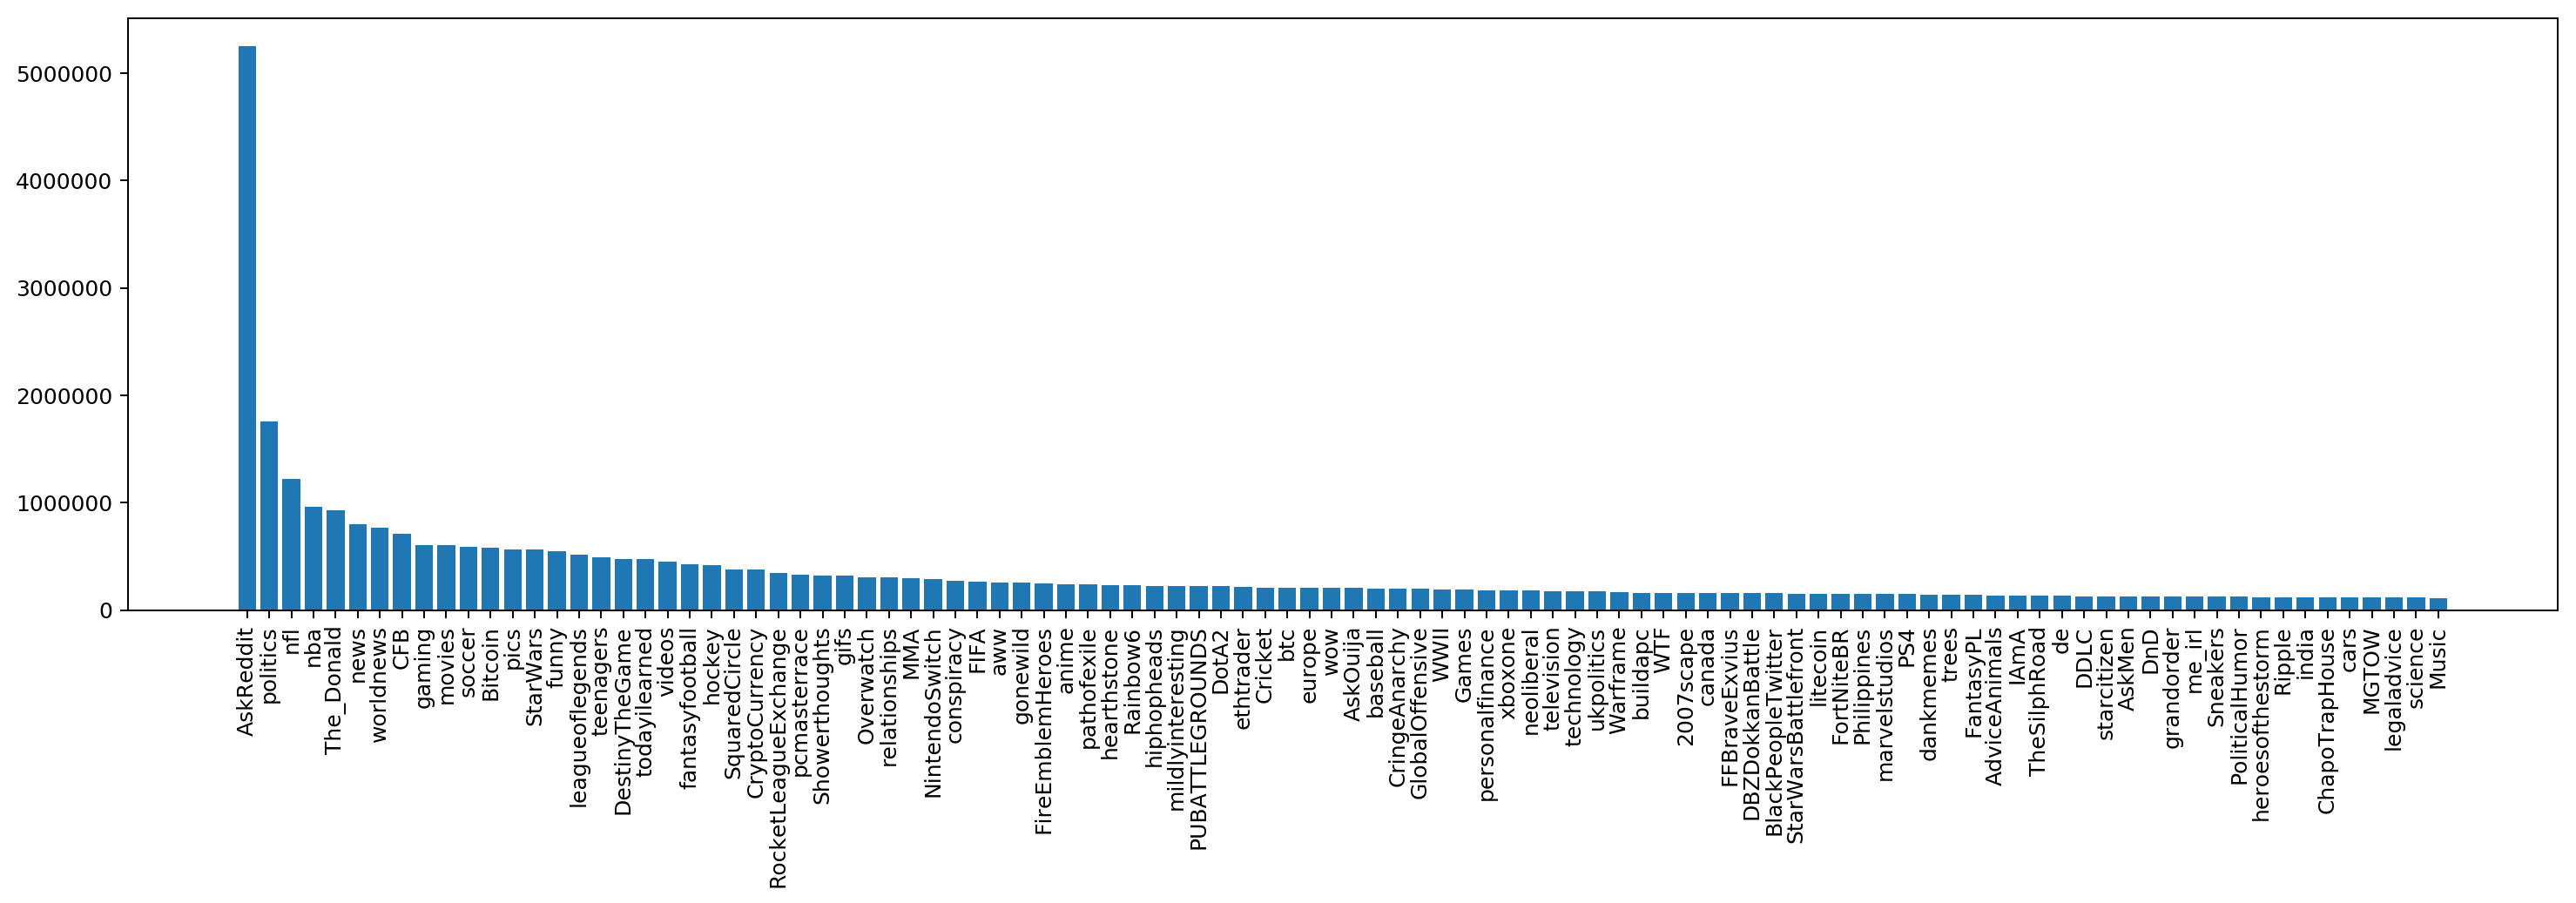
\includegraphics[width=\linewidth]{subreddit_activity.png} \\
\caption{Most active subreddits by number of comments in December 2017}
\label{fig:hist}
\end{figure}

Since processing such dataset was unfeasible on a standard desktop we decided to
take a sample of it by keeping each comment in the original dataset with a
probability of $\frac{1}{8}$ and transforming the format from JSONLine to csv
which reduces the space needed for storage.


\section{Mobilization Sentiment Prediction through LSTM}
\label{sec:davide}

The author's dataset was built with the help of Mechanical Turk crowdworkers
that manually annotated almost a thousand of cross-links telling whether the
sentiment of the source post towards the target post was negative or
positive/neutral reaching a inter-rater agreement of 0.95. Over this sample the
authors applied a Random Forest classifier with forests of 400 trees that
achieves an accuracy of 0.80 on a 10-fold cross validation. They then used this
classifier to build the dataset presented in Section \ref{sec:intro}. Such
dataset was used as a ground
truth to train our model. By performing the retrieval described above we
obtained a set of instances of which about 95\% labeled as positive as
announced in the original paper raising another challenge. Such unbalancing
between the number of
instances of the classes would produce an unreliable evaluation therefore we
chose to undersample the retrieved dataset. Instead of using a random heuristic
we used the NearMiss version 1 method that reduces the number of positive
elements by keeping only those positive instances for which the average distance
to the N closest samples of the negative class is the smallest. After
undersampling we obtain a dataset of about 8,000 instances that is split into
80\% of training set and 20\% of test set.

Instead of employing the large set of features, that by the way are not
very well documented, used by the authors in this setting we propose an improved
model based on the bare content of the post and its comments in terms of
contained words. This is a trend in modern classification methods
where deep learning models substitute annoying feature engineering.


Our model is essentially based on a combination of a convolutional
neural network followed by a LSTM recurrent network. At the basis of the model we
use GloVe word embeddings that allow us to represent each word in the text in a fixed-
size, compact and dense vector of 300 floats also taking into account
similarities between
words. The advantage of GloVe vectors over the simple one-hot representation of words
is that these vectors were trained using a neural network so that words that have a
similar context are close in the vector space. Then the word embeddings are given in 
input to the convolutional layer. The purpose
of this layer is to capture more general patterns in the data helping the network to better
generalize to new examples without excessively specialising on the text of the training
data. The result is given in input to the bidirectional LSTM layer which is responsible
of learning the patterns in the sequences of words, something that recurrent network
were designed to do well. In particular the LSTM architecture allows to ”remember”
longer sequences learning which parts of the sequences are more important. After
some tuning of the hyperparameters we obtained a classifier with an accuracy of
0.90, significantly above from the baseline of the reference paper, and the
following performances.

\begin{verbatim}
             precision    recall  f1-score   support

  non-burst       0.87      0.93      0.90       769
      burst       0.93      0.87      0.90       807

  avg/total       0.90      0.90      0.90      1576
\end{verbatim}

\section{Attacker Defender PageRank}

To understand whether in the target post of a negative mobilization attackers
and defenders talk to each other or they form their own groups thus creating
echo chambers we construct a graph of the users' interactions. The reply network
was extracted using the structure of the comments in Reddit posts where a
comment can be in response to another comment. In particular each node is a user,
either attacker or defender, and a directed edge from user $i$ to user $j$
indicates that $i$ replied to one of $j$'s comment. The weight of the edge
indicates the number of times a user replied. Such network is constructed for
each of the target post of the negative mobilizations in a sample of the dataset
provided by the authors.

We quantify the echo chamber by replicating the approach of the paper which is
based in the application of personalized PageRank: firstly by restricting the
teleport set to the defender nodes (Defender PageRank) and secondly to the
attacker nodes (Attacker PageRank). The Defender PageRank (resp. Attacker
PageRank) score of a node represents its centrality measured from the perspective
of Defender nodes (resp. Attacker nodes).

We noted that in many networks the number of defenders dominated the number of
attackers as expected by the fact that the target post attracts more the
interest of users of that subreddit than a cross-link mobilizes the users of the
source subreddit. Still an important portion (83\%) of defenders has a 0.0 PageRank
implying that only a subset of the community gets involved in controversial
conversations.

Finally as done in the reference paper we have computed the average of the
PageRank scores of attackers and defenders in Attacker PageRank and Defender
PageRank considering all the networks. As highlighted in the paper
attackers have a significantly higher score than defenders in Attacker PageRank,
which is an evidence of echo chambers in the attacker's group that result in
non-constructive discussions. Differently from the reference paper we obtained a
high score for the attackers also in the Defender PageRank which might be caused
by the number of considered networks.


\begin{figure}[h]
\centering
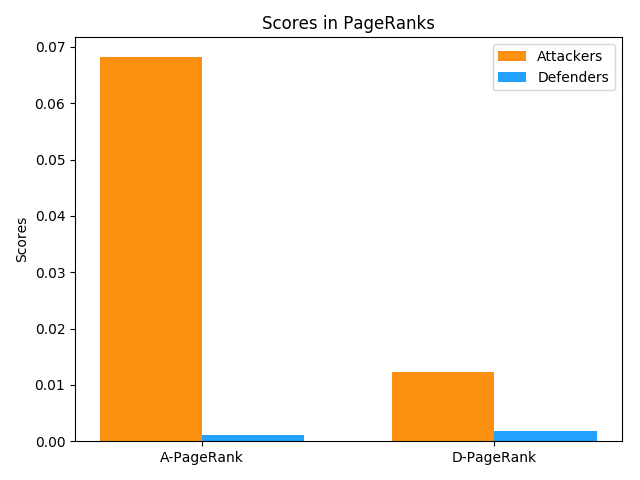
\includegraphics[width=0.4\linewidth]{hist.png} \\
\caption{Average of Attacker PageRank and Defender PageRank for attackers and
defenders}
\label{fig:hist}
\end{figure}

\section{Recommender System}

Interested in the properties of the reddit social network, we decided to extend
the analysis provided in the reference paper by trying to implement a
subreddit recommender system. In order
to implement such system we preferred to not perform a crawl of the reddit
website since it could have produced a bias in the result coming from the fact
that the communities are not necessarily linked. Instead we chose to use the
sample of the reddit comments of December 2017 retrieved as explained in Section
\ref{sec:retrieval}. This is of course an over-semplification of the task but it
is based in the often valid assumption that contents of subreddits do not change
rapidly at the granularity of the month.

The first phase of the design process was to choose how to tackle the problem.
We thought about experimenting a Collaborative Filtering approach but the amount
of users in the sample and the sparsity of user-subreddit matrix would have not
been significantly effective. Instead we opted for a Content-Based system using
subreddit similarities. We chose to focus only on the top-5000 most active
subreddits and to represent a subreddit as the TF-IDF vector
of the most frequent words in its comments. We split the computation into
multiple phases. In the first phase we grouped comments by subreddit. In the
second phase we tokenized the comments, removed stop words and performed
stemming based on the Porter algorithm. Finally we computed the TF-IDF vector of
length 20,000 for each subreddit by considering a vocabulary with the 20,000
terms having the highest TF.

The recommender system was tested on a sample of 258,050 users whose comments
were not used for the TF-IDF computations. We evaluated two approaches in the
recommendation. In both cases the recommender system was given in input the
two subreddits in which the user has commented the most. In the first approach
the system recommends the first $k$ subreddits that are the most similar to the
ones taken as input according to the cosine similarity metric. In the second
approach, the user is represented as the mean of the two subreddits and the
$k$ subreddits recommended are the ones having highest cosine similarity score
with respect to the user vector.

We decided to recommend 5 subreddits and consider as relevant all the subreddit
the user commented on. The choice of limiting the number of recommended
subreddits was given by the scarcity of comments. The system performances are
presented below.

\begin{figure}[h]
\centering
\includegraphics[width=0.5\linewidth]{precrec.png} \\
\caption{Precision and Recall @$k$ for $k \in \{1 .. 5\}$ for the two methods
computed as average over all the users}
\label{fig:hist}
\end{figure}

\section{Conclusion}

We have analyzed the reddit social network and found interesting results of the
interactions and similarities between communities. The process was full of
difficulties and edge cases given the characteristics of the problem and the
structure of the social network. We faced the problem of rate limiting of the
APIs, of processing large amounts of data on small machines and resolved
problems in the distribution of the dataset. We dipped our feet in the design of
a naive recommender system facing to choose the criteria for recommendation, the
number of subreddits to receive as input and to recommend constrained by the scarcity
of comments per user in a month of data.

Overall this was an interesting project since it allowed us to face real
problems and not apply only well studied algorithms in well-crafted datasets.

\section*{References}

\small

[1] Srijan Kumar, William L. Hamilton, Jure Leskovec, and Dan Jurafsky. Community Interaction and Conflict on the Web. The Web Conference (WWW). 2018.

\end{document}
